\section{Chapter 1 Problems}
\graphicspath{{figures/chapter1/}}
\subsection{Problem 1.21}
\begin{lstlisting}
> p1.21.x=(-5:5)
> p1.21.y <- 4*p1.21.x - 4
> plot(p1.21.x, p1.21.y, xlab = 'X', ylab = 'Y', 
+ main = "Problem 1.21", sub = "Plot of Y = 4*X - 4")
> abline(line(p1.21.x, p1.21.y))
\end{lstlisting}
	See Figure \ref{p1.21}
	\begin{figure}[!htb]
	  \centering
	  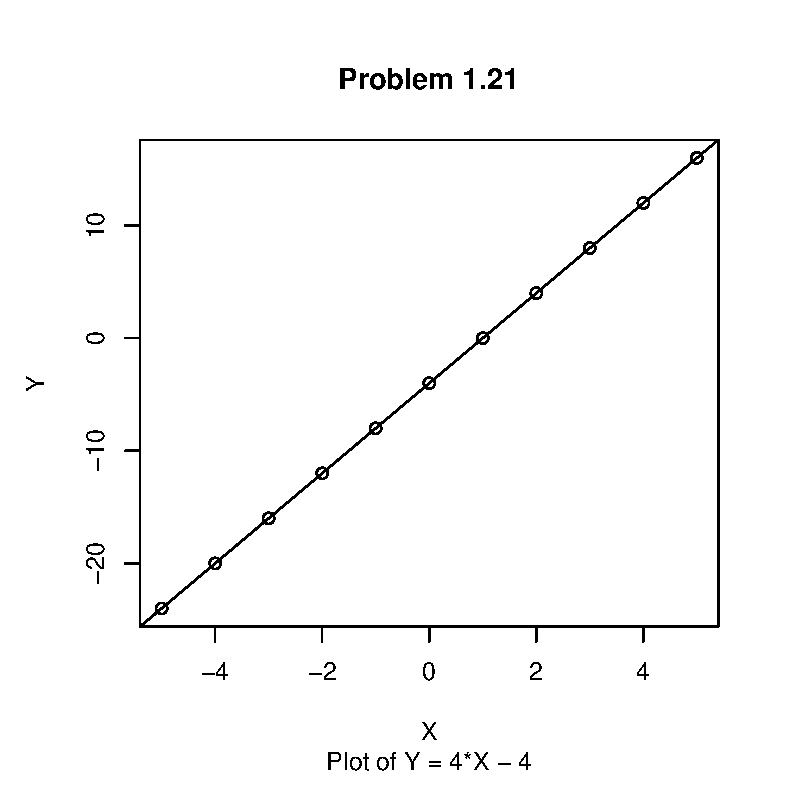
\includegraphics[width=0.5\textwidth]{p1.21.eps}
	  \caption{Problem 1.21 \label{p1.21}}
	\end{figure}

\subsection{Problem 1.22}
\begin{lstlisting}
> p1.22.x <- (-5:5)
> p1.22.y <- 2 * p1.22.x ^ 2 - 3 * p1.22.x - 9
>  plot(p1.22.x, p1.22.y, xlab = "X", ylab = "Y",
+ main = expression(Y == 2*X^2 - 3*X - 9))
> curve(2*x^2 - 3*x - 9, add = TRUE)
\end{lstlisting}
	See Figure \ref{p1.22}
	\begin{figure}[!htb]
	  \centering
	  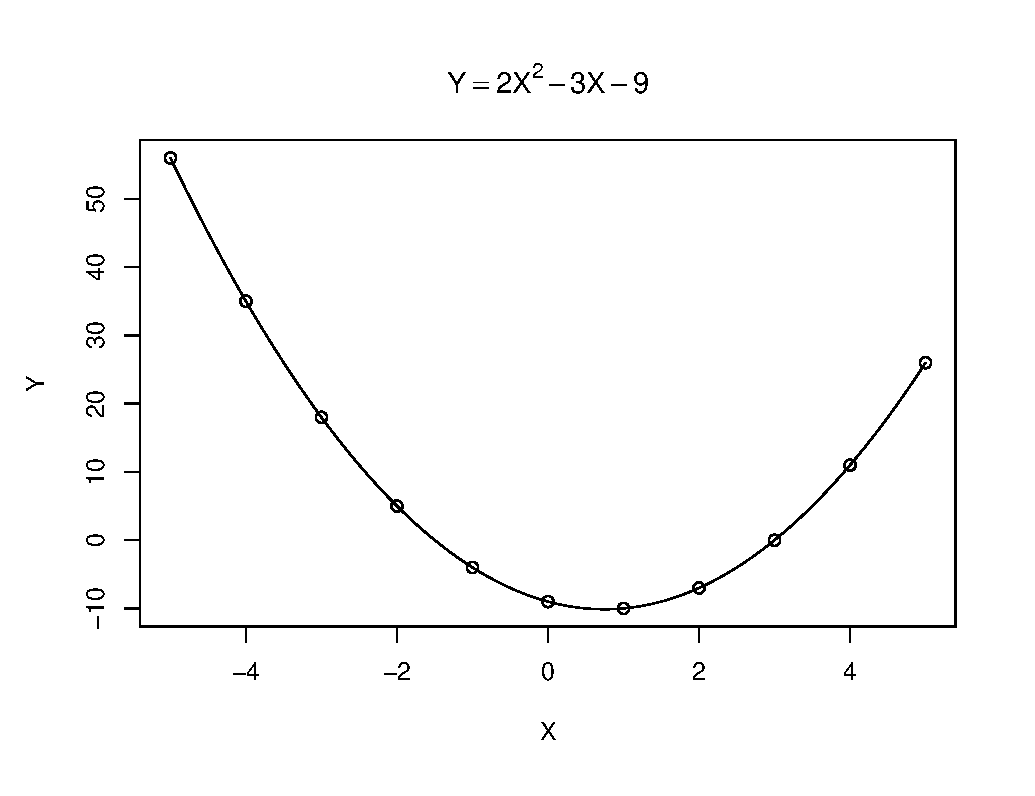
\includegraphics[width=0.5\textwidth]{p1.22.eps}
	  \caption{Problem 1.22 \label{p1.22}}
	\end{figure}

\subsection{Problem 1.23}
\begin{lstlisting}
> p1.23.x <- (1997:2005)
> p1.23.y = c(0.88, 0.90, 1.01, 1.10, 1.2, 1.25, 1.28, 1.36, 1.41)
> par(mfcol = c(1,2))
> plot(p1.23.x, p1.23.y, xlab = "Year", ylab = "Millions",
+ main = "Number of New Diabetes Diagnosed")
> lines(p1.23.x, p1.23.y)
> barplot(p1.23.y, names.arg = p1.23.x, xlab = "Year", ylab = "Millions",
+ main = "Number of New Diabetes Diagnosed", space = 1.5)
\end{lstlisting}
	See Figure \ref{p1.23}
	\begin{figure}[!htb]
	  \centering
	  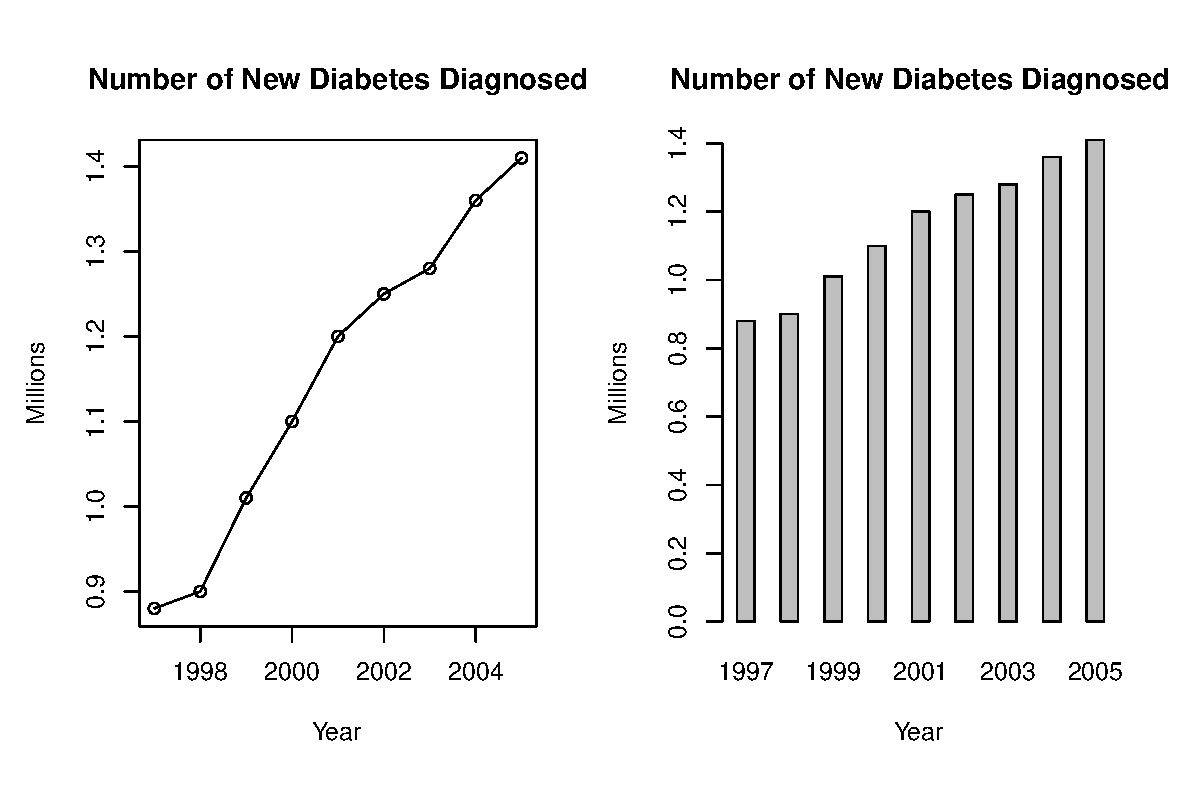
\includegraphics[width=0.9\textwidth]{p1.23.eps}
	  \caption{Problem 1.23 \label{p1.23}}
	\end{figure}

\subsection{Problem 1.28}
\begin{lstlisting}
> p1.28 <- c(2, 15, 29, 26, 16, 12)
> names(p1.28) <- c("None", "One", "Two", "Three", "Four", "Five +")
> pie(p1.28, main = "Number of Televisions in American Households")
\end{lstlisting}
	See Figure \ref{p1.28}
	\begin{figure}[!htb]
	  \centering
	  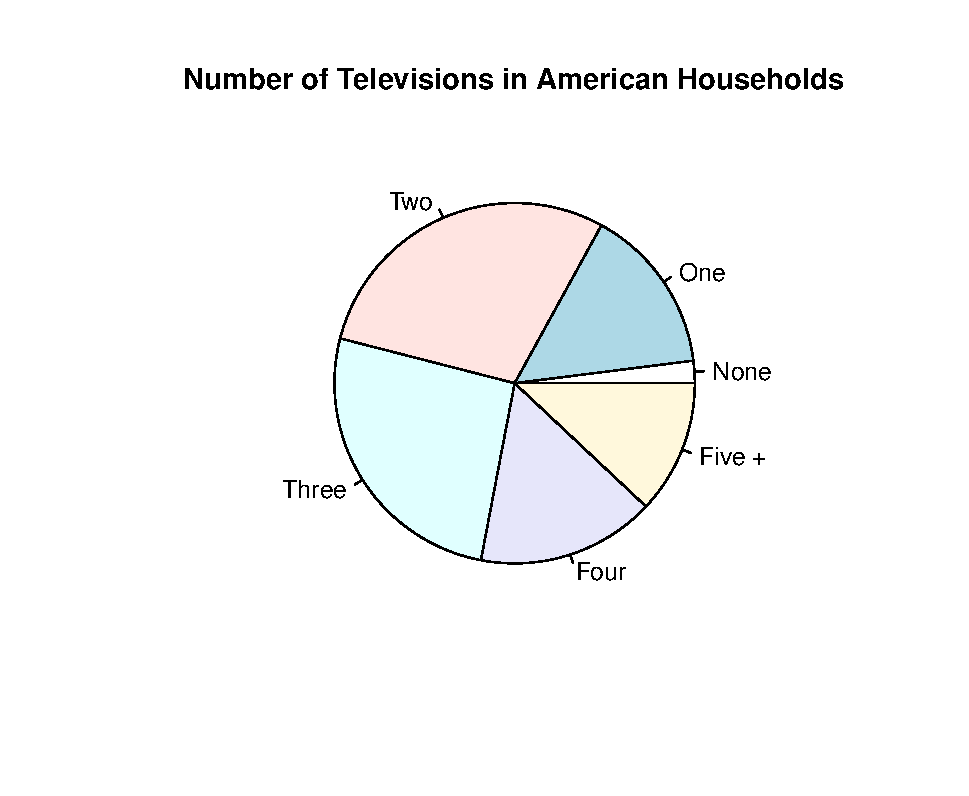
\includegraphics[width=0.7\textwidth]{p1.28.eps}
	  \caption{Problem 1.28 \label{p1.28}}
	\end{figure}

%\clearpage

\subsection{Problem 1.63}
\begin{lstlisting}
> p1.9.data = read.table("data/1.9.data", header = TRUE, sep = ',')
> par(mfcol = c(1,2))
> plot(p1.9.data$Year, p1.9.data$Clubs, xlab = 'Year', 
+ ylab = 'clubs', main = 'Number of Health Clubs by Year', type = 'b')
> plot(p1.9.data$Year, p1.9.data$Members, xlab = 'Year', 
+ ylab = 'Members', main = 'Number of Health Club Members by Year',
+ type = 'b')
\end{lstlisting}
	See Figure \ref{p1.63}
	\begin{figure}[!htb]
	  \centering
	  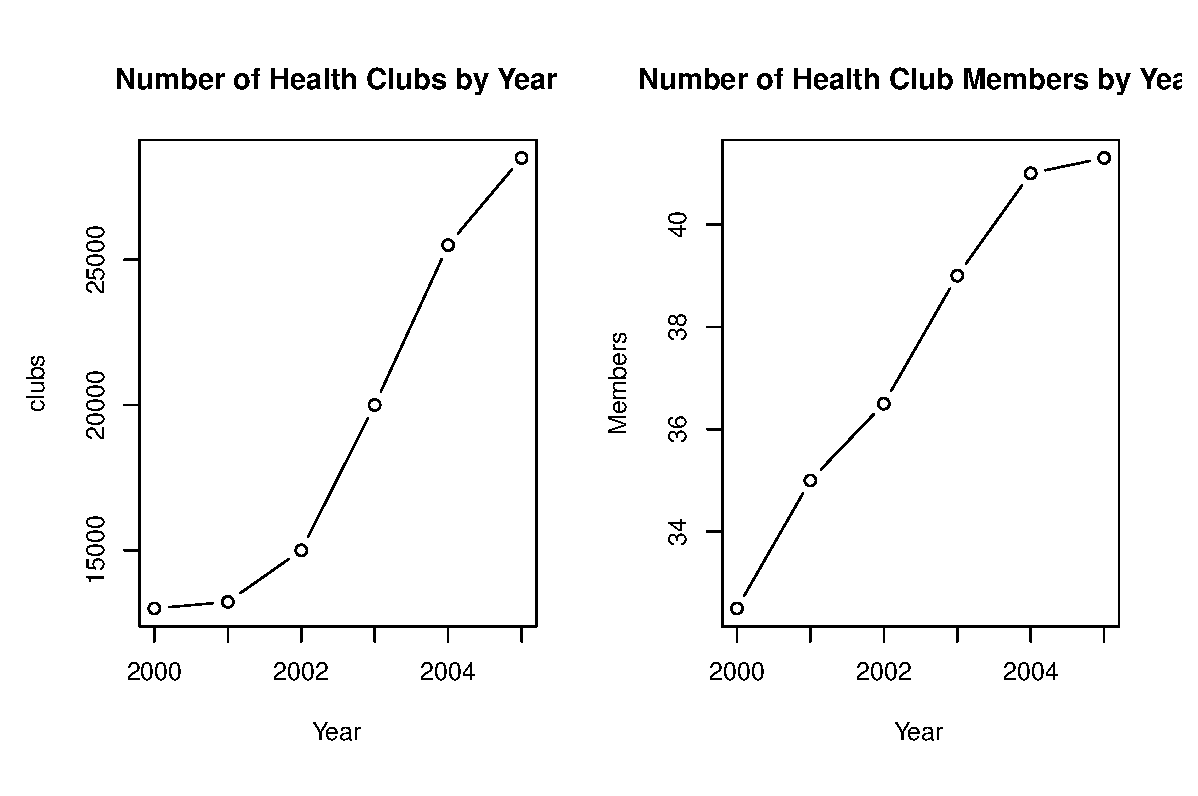
\includegraphics[width=0.8\textwidth]{p1.63.eps}
	  \caption{Problem 1.63 \label{p1.63}}
	\end{figure}
	
\clearpage

\subsection{Problem 1.64}
\begin{lstlisting}
> # cont...
> barplot(p1.9.data$Clubs, names.arg = p1.9.data$Year, xlab = 'Year', 
+ ylab = 'Clubs', main = 'Health Clubs by Year')
> barplot(p1.9.data$Members, names.arg = p1.9.data$Year, xlab = 'Year', 
+ ylab = 'Members', main = 'Health Club Members by Year')
\end{lstlisting}
	See Figure \ref{p1.64}
	\begin{figure}[!htb]
	  \centering
	  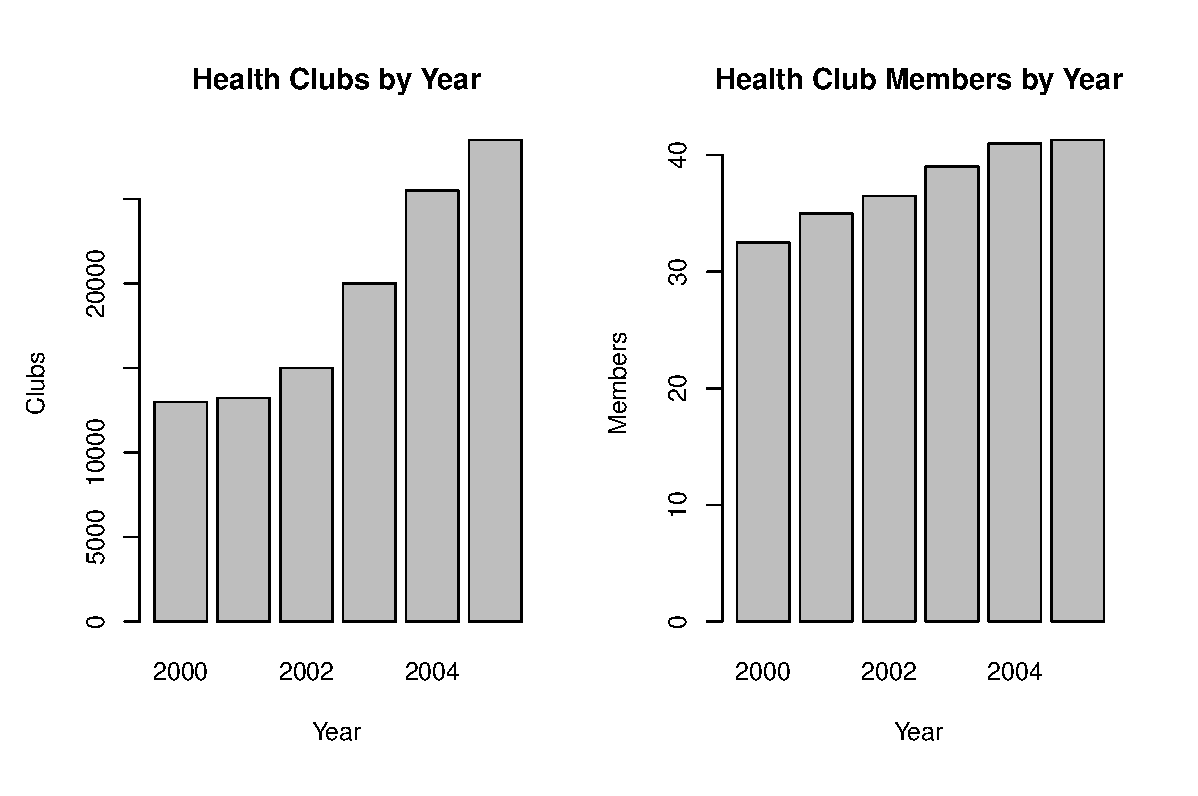
\includegraphics[width=0.9\textwidth]{p1.64.eps}
	  \caption{Problem 1.64 \label{p1.64}}
	\end{figure}

\subsection{Problem 1.65}
\begin{lstlisting}
> attach(p1.9.data)
> plot(Clubs, Members, main = 'Clubs to Members (mil)')
\end{lstlisting}
	See Figure \ref{p1.65}
	\begin{figure}[!htb]
	  \centering
	  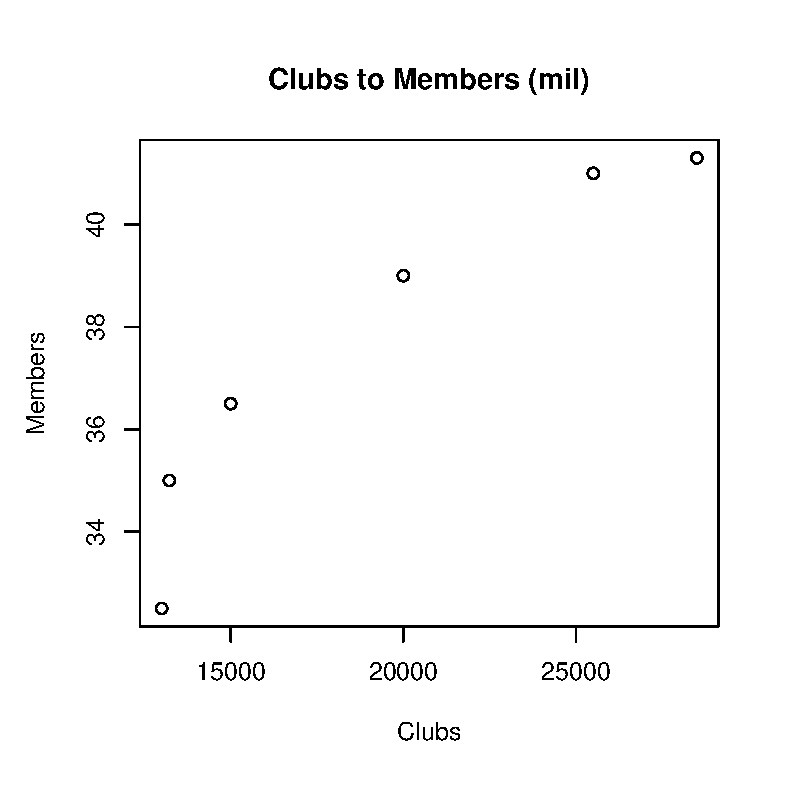
\includegraphics[width=0.5\textwidth]{p1.65.eps}
	  \caption{Problem 1.65 \label{p1.65}}
	\end{figure}

\subsection{Problem 1.70}
\begin{lstlisting}
> p1.70.data = read.csv("data/1.70.csv")
> {attach(p1.70.data); op <- par(mfcol = c(1,2))}
> pie(Male, labels = Marital.Status, main = 'Male')
> pie(Female, labels = Marital.Status, main = 'Female')
> {detach(1p.70.data); par(op)}
\end{lstlisting}
	See Figure \ref{p1.70}
	\begin{figure}[!htb]
	  \centering
	  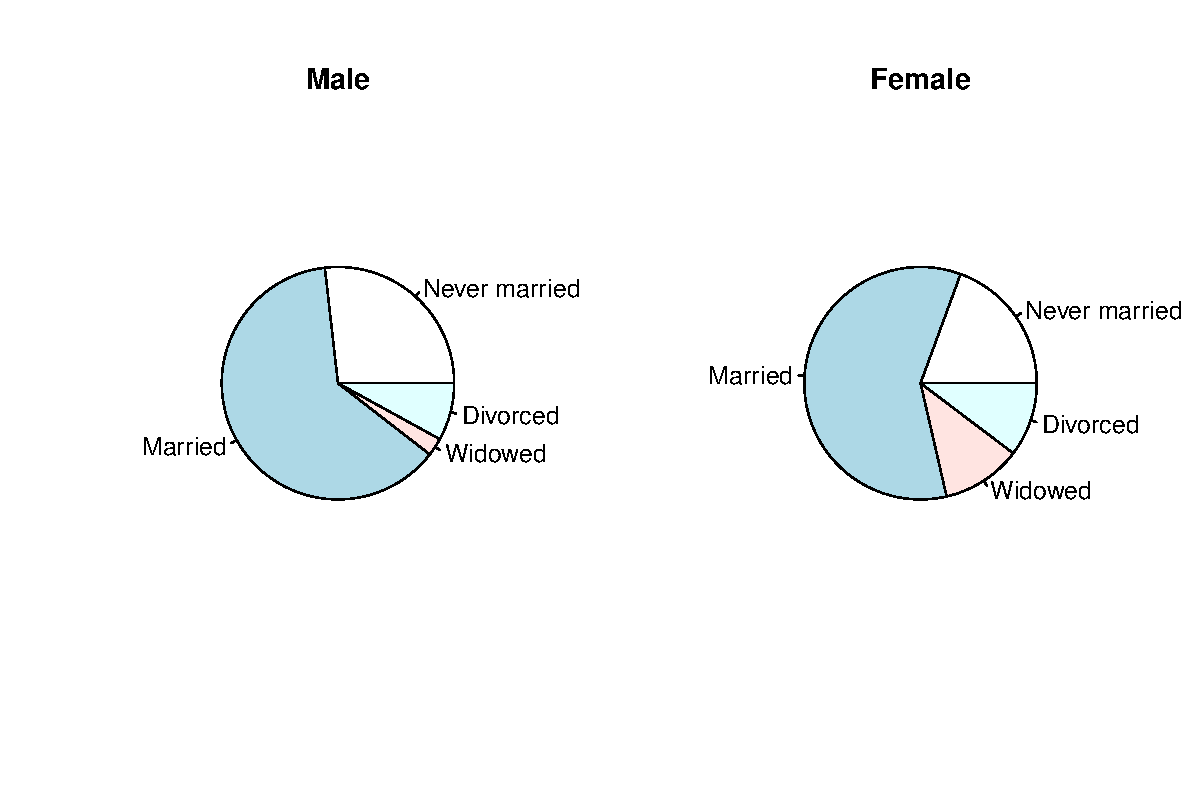
\includegraphics[width=0.9\textwidth]{p1.70.eps}
	  \caption{Problem 1.70 \label{p1.70}}
	\end{figure}

\clearpage